% Standalone two-column-wide system diagram for Fig. 1, revision 1.
% Compile:  pdflatex fig1_system_r1.tex -> fig1_system_r1.pdf (place in fig/)
%
% Changes over fig1_system.tex (Reviewers 2.9 and 5.7):
%  - blue for the shared path and orange for the private path, the pair
%    that survives the common forms of colour vision deficiency. Grouping
%    regions and the offline support blocks are grey shaded, the offline
%    blocks keeping a dashed edge so they stay separable from the online
%    chain in greyscale.
%  - the smoothing acronym no longer appears, since the figure precedes
%    the section that defines it.
\documentclass[tikz,border=3pt]{standalone}
\usetikzlibrary{arrows.meta,positioning,fit,calc,backgrounds}
\usepackage{bm}
\usepackage{amsmath,amssymb}

\begin{document}
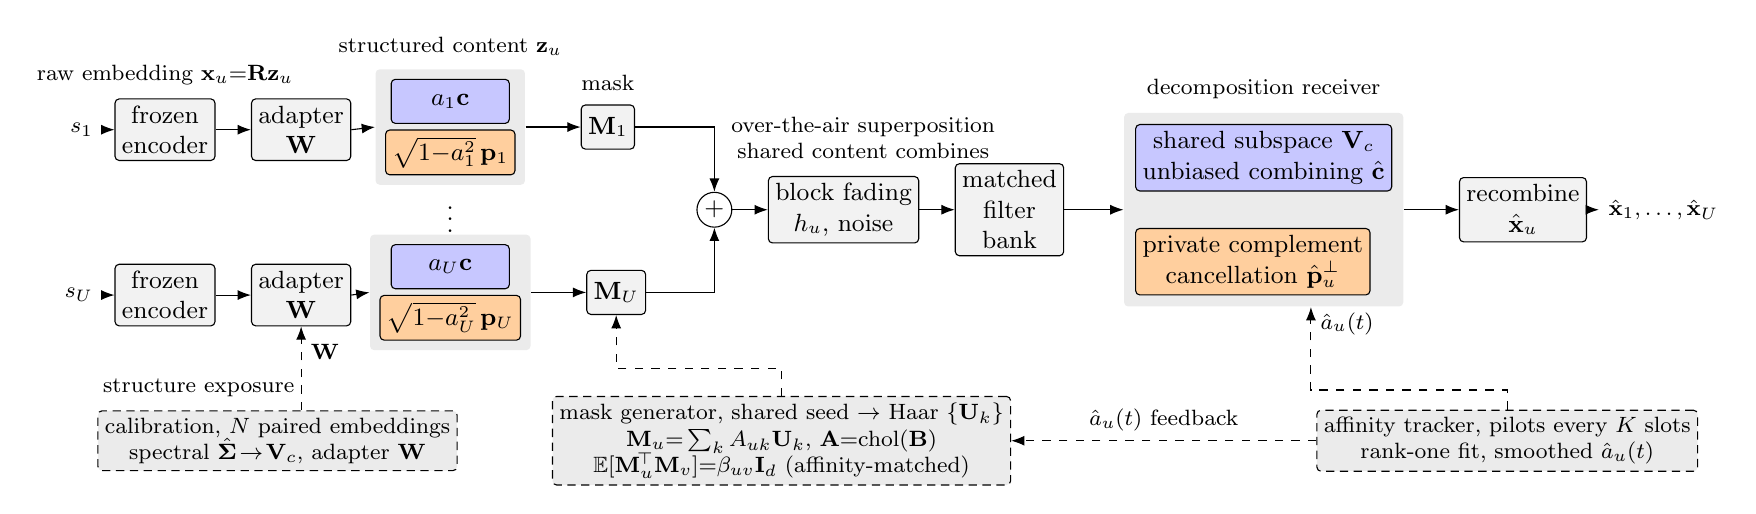
\begin{tikzpicture}[font=\small,>=Latex,
  box/.style={draw,rounded corners=1.5pt,minimum height=5.6mm,inner sep=2.5pt,
              fill=gray!10,align=center},
  shared/.style={box,fill=blue!22},
  priv/.style={box,fill=orange!38},
  aux/.style={box,fill=black!8,densely dashed,font=\footnotesize},
  lbl/.style={font=\footnotesize},
  grp/.style={fill=black!8,rounded corners=1.5pt,inner sep=1.2mm}]

% ================= user 1 chain =================
\node[box] (enc1) at (0,1.05) {frozen\\encoder};
\node[lbl,left=1.5mm of enc1] (s1) {$s_1$};
\node[box,right=4.5mm of enc1] (w1) {adapter\\$\mathbf{W}$};
\node[shared,right=5mm of w1,yshift=3.6mm,minimum width=15mm]
  (sh1) {$a_1\mathbf{c}$};
\node[priv,below=0.7mm of sh1,minimum width=15mm]
  (pr1) {$\sqrt{1{-}a_1^2}\,\mathbf{p}_1$};

% ================= user U chain =================
\node[box] (enc2) at (0,-1.05) {frozen\\encoder};
\node[lbl,left=1.5mm of enc2] (s2) {$s_U$};
\node[box,right=4.5mm of enc2] (w2) {adapter\\$\mathbf{W}$};
\node[shared,right=5mm of w2,yshift=3.6mm,minimum width=15mm]
  (sh2) {$a_U\mathbf{c}$};
\node[priv,below=0.7mm of sh2,minimum width=15mm]
  (pr2) {$\sqrt{1{-}a_U^2}\,\mathbf{p}_U$};

% ================= embedding groups and masks =================
\begin{scope}[on background layer]
\node[grp,fit=(sh1)(pr1)] (emb1) {};
\node[grp,fit=(sh2)(pr2)] (emb2) {};
\end{scope}
\node[box,right=7mm of emb1] (m1) {$\mathbf{M}_1$};
\node[box,right=7mm of emb2] (m2) {$\mathbf{M}_U$};

\node at ($(emb1.south)!0.5!(emb2.north)+(0,-0.02)$) {$\vdots$};
\node[lbl,above=0.5mm of emb1,align=center]
  {structured content $\mathbf{z}_u$};
\node[lbl,above=0.5mm of enc1,align=center]
  {raw embedding $\mathbf{x}_u{=}\mathbf{R}\mathbf{z}_u$};
\node[lbl,above=0.5mm of m1,align=center] {mask};

% ================= channel =================
\node[draw,circle,inner sep=1.1pt] (sum) at ($(m1)!0.5!(m2)+(13mm,0)$) {$+$};
\node[box,right=4.5mm of sum,align=center] (ch) {block fading\\$h_u$, noise};
% offset so the label clears the vertical arrow into the summation node
% on its left and the matched-filter block below its right end
\node[lbl,above=1mm of ch,xshift=2.5mm,align=center]
  {over-the-air superposition\\shared content combines};

% ================= receiver =================
\node[box,right=4.5mm of ch,align=center] (mf) {matched\\filter\\bank};
\node[shared,right=9mm of mf,yshift=6.6mm,minimum width=29mm,align=center]
  (comb) {shared subspace $\mathbf{V}_c$\\unbiased combining $\hat{\mathbf{c}}$};
\node[priv,right=9mm of mf,yshift=-6.6mm,minimum width=29mm,align=center]
  (canc) {private complement\\cancellation $\hat{\mathbf{p}}_u^{\perp}$};
\begin{scope}[on background layer]
\node[grp,inner sep=1.4mm,fit=(comb)(canc)] (dr) {};
\end{scope}
\node[lbl,above=0.5mm of dr,align=center] {decomposition receiver};
\node[box,align=center,right=7mm of dr] (rec)
  {recombine\\$\hat{\mathbf{x}}_u$};
\node[lbl,right=1.5mm of rec] (out) {$\hat{\mathbf{x}}_1,\dots,\hat{\mathbf{x}}_U$};

% ================= bottom row: exposure, mask generator, tracker ==========
\node[aux,align=center] (cal) at ($(w1)!0.5!(w2)+(-3mm,-29mm)$)
  {calibration, $N$ paired embeddings\\spectral
   $\hat{\bm{\Sigma}}\!\rightarrow\!\mathbf{V}_c$, adapter $\mathbf{W}$};
\node[lbl,above=0.5mm of cal,align=center,xshift=-10mm]
  {structure exposure};
\node[aux,align=center] (mgen) at ($(m2.south |- 0,0)+(21mm,-29mm)$)
  {mask generator, shared seed $\rightarrow$ Haar $\{\mathbf{U}_k\}$\\
   $\mathbf{M}_u{=}\textstyle\sum_k A_{uk}\mathbf{U}_k$,
   $\mathbf{A}{=}\mathrm{chol}(\mathbf{B})$\\
   $\mathbb{E}[\mathbf{M}_u^{\!\top}\mathbf{M}_v]{=}\beta_{uv}\mathbf{I}_d$
   (affinity-matched)};
\node[aux,align=center] (trk) at ($(rec.south |- 0,0)+(-2mm,-29mm)$)
  {affinity tracker, pilots every $K$ slots\\rank-one fit,
   smoothed $\hat{a}_u(t)$};

% ================= arrows =================
\draw[->] (s1) -- (enc1);
\draw[->] (s2) -- (enc2);
\draw[->] (enc1) -- (w1);
\draw[->] (enc2) -- (w2);
\draw[->] (w1.east) -- (emb1.west);
\draw[->] (w2.east) -- (emb2.west);
\draw[->] (emb1.east) -- (m1.west);
\draw[->] (emb2.east) -- (m2.west);
\draw[->] (m1.east) -| (sum.north);
\draw[->] (m2.east) -| (sum.south);
\draw[->] (sum) -- (ch);
\draw[->] (ch) -- (mf);
\draw[->] (mf.east) -- (dr.west);
\draw[->] (dr.east) -- (rec.west);
\draw[->] (rec) -- (out);
% offline exposure path (adapter update)
\draw[->,dashed] (cal.north -| w2) --
  node[lbl,right,pos=0.7]{$\mathbf{W}$} (w2.south);
% mask generation path
\draw[->,dashed] (mgen.north) -- ++(0,3.5mm) -| (m2.south);
% tracker path to the decomposition receiver
\draw[->,dashed] (trk.north) -- ++(0,2.5mm) -|
  node[lbl,right,pos=0.9]{$\hat{a}_u(t)$} ($(dr.south)+(6mm,0)$);
% affinity feedback bus to the mask generator
\draw[->,dashed] (trk.west) |-
  node[lbl,above,pos=0.75]{$\hat{a}_u(t)$ feedback} (mgen.east);
\end{tikzpicture}
\end{document}
